% binary search - painting (sort buckets and binary search), money, careful ascent

\section{Binary Search}
\begin{frame}{}{}
  \begin{center}
    {\bf Part III: Binary Search}
  \end{center}
\end{frame}

\begin{frame}
  \frametitle{Divide and Conquer Idea}

  The Bynary Search algorithm is based on the idea of {\bf Divide and Conquer}
  (D\&C).\bigskip

  D\&C means to make a problem simple by dividing it in smaller parts.
  It is easier to solve the smaller parts than the big one.
  \bigskip

  \begin{block}{Examples of algorithms using D\&C approach}
    Binary Search, Quick Sort, Merge Sort, many algorithms on Tree Graphs, etc...
  \end{block}
\end{frame}

\begin{frame}{Binary Search Algorithm}

  You want to find number $k$ in a very large array $A$ of size $n$:
  \bigskip

  \begin{enumerate}
  \item Sort $A$; Set begin = 0; End = $n$
  \item Test $a_{(end - begin)/2}$ (The middle of begin and end)
  \item If $a_{(end - begin)/2} > k$, $end = end - begin / 2$
  \item If $a_{(end - begin)/2} < k$, $begin = end - begin / 2$
  \item Go to 2 until you find k
  \end{enumerate}\bigskip

  The search time is $O(n\log n)$ (sorting) + $O(\log n)$ for each search.\bigskip

  If the number of searches is (very) small, it is better to just loop the array.\bigskip

  If the number of searches is big, or if the array is sorted in the beginning,
  it is better to use binary search.
\end{frame}

\subsection{Example Problem}
\begin{frame}{Binary Search Problem: Room Painting}
  \begin{block}{Problem Description}
    \begin{itemize}
      \item Input: $n < 100.000$ can sizes and $m < 100.000$ paint sizes, in random order.
      \item For each paint size $m_i$, find the smallest $n_j$ so that $n_j > m_i$.
    \end{itemize}
  \end{block}

  {\bf Full Search Solution}: Loop $m$ times around $n$ -- simple to code, but total cost is $O(m*n) = 10.000.000.000$.\bigskip

  {\bf Binary Search Solution}: Sort $n$, then do binary search $m$ times. Total cost is:\\
  $O(n\log n) + O(m\log n) \approx 200.000 * 11 \approx 2.000.000$.\bigskip

  Remember you can use the "upper\_bound" function in C++. No need to code by hand.


\end{frame}

\subsection{Binary Search for Simulation}

\begin{frame}{Binary Search for Simulation}
  You can also use Binary Search to calculate complicated calculations.\bigskip

  \begin{itemize}
    \item Consider the complicated function $f(x)$;
    \item You want to find $x'$ so that $f(x') = 0$;
    \item Estimate $x_{min}$ and $x_{max}$;
    \item Do a {\bf Binary Search} between $x_{min}$ and $x_{max}$, using $f(x)$ to test.
  \end{itemize}\bigskip


  \begin{block}{}
    Note: This approach only works if the calculation is {\bf monotonic}.
  \end{block}
\end{frame}


\begin{frame}
  \frametitle{Example 1: Paying a Debt}

  \begin{block}{Problem Description}
    \begin{itemize}
      \item Pay a total of $V$. You pay $D$ per month, for $M$ months.
      \item Each month $V$ increases before paying, $V = V * i$.
      \item Given $M$,$i$ and $V$, what is the minimum $D$?
    \end{itemize}
  \end{block}
  \bigskip

  $V = 1000$, $M = 2$, $i = 1.1$, what is the minimum $D$?

  \begin{itemize}
  \item if $D = 500$:
    \begin{itemize}
    \item $m_1: V_0 * 1.1 - D = 600, m_2: V_1 * 1.1 - D = 160$: D is too small
    \end{itemize}
  \item if $D = 600$:
    \begin{itemize}
    \item $m_1: V_0 * 1.1 - D = 500, m_2: V_1 * 1.1 - D = -50$: D is too big
    \end{itemize}
  \end{itemize}
\end{frame}


\begin{frame}{Example 1: Paying a Debt with Binary Search}

\begin{itemize}
  \item Input: $m = 2, v = 1000, i = 1.1$
  \item Choose initial range: (ex: [0.01 to 1100.00]); Initial $d$: 550.005
  \item $f(d,m,v,i) = \text{loop}(v*i - d)$, $m$ times
  \item Do binary search in this range;
\end{itemize}
\bigskip

{\smaller
\begin{tabular}{c|c|c|c|l}
 a & b & d & simulation: f(d,m,v,i) & action: \\
 \hline
 0.01 & 1100.00 & 550.005 & error: -54.98 & increase a\\
 550.005 & 1100.00 & 825.002 & error: 522.50 & decrease b\\
 550.005 & 825.002 & 687.503 & error: 233.75 & decrease b\\
 550.005 & 687.503 & 681.754 & error: 89.38 & decrease b\\
 550.005 & 618.754 & 584.379 & error: 17.19 & decrease b\\
 550.005 & 584.379 & 567.192 & error: -18.89 & increase a\\
 567.192 & 584.379 & 575.786 & error: -0.84 & increase a\\
 ... & ... & ... & a few iterations later ... & ...\\
 ... & ... & 576.190 & error $< \epsilon$ & stop: answer = 576.19\\
\end{tabular}}
\bigskip

Total number of steps: $O(log_2((b-a)/\epsilon))$ \hfill{\bf Attention: Choose a stop criteria carefully!}
\end{frame}

\begin{frame}{Binary Search in a Simulation, Example 2: carefulascent}
  \begin{itemize}
    \item Given the position of the ship $(x,y)$, and a fixed vertical speed ($v = 1$),
    \item Find horizontal speed ($h$)
    \item There are $n$ shields that change the horizontal speed.
    \item Acceptable error: $10^6 = 0.000001$; calculate with more digits than this.
  \end{itemize}
  \begin{center}
    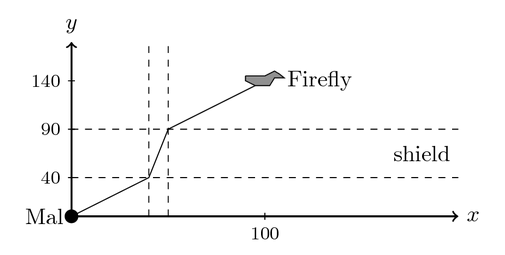
\includegraphics[width=0.6\textwidth]{img/carefulascent.png}
    \ppagenote{Careful Ascent Image CC-BY-SA, from Egor Dranischnikow}
  \end{center}
\end{frame}
